\chapter{Análise Bibliográfica sobre Simulação Multiagente e Fenômenos Sociais, por Jorge Fernandes\label{chap:bibliometria:jhcf}}

\section{Planejamento do estudo}
O planejamento o  desenho do estudo deve descrever as motivações, questões de interesse, escopo, limitações e objetivos do trabalho.

O planejamento do estudo deve motivar o tema escolhido e o interesse do autor.

No caso do meu trabalho, as perguntas que o nortearam foram:
\begin{itemize}
    \item Qual a base de conhecimentos científicos produzida em torno do tema simulação multiagente voltada à compreensão de fenômenos sociais, com ênfase em métodos experimentais? 
    \item Como a simulação multiagente tem sido usada para compreender fenômenos sociais, com ênfase em métodos experimentais? 
    \item Quais os principais termos e conceitos ligados à frente de pesquisa no tema simulação multiagente de fenômenos sociais, com ênfase em métodos experimentais? 
    \item Qual a estrutura social da comunidade, se é que existe, que pesquisa sobre o tema simulação multiagente de fenômenos sociais, com ênfase em métodos experimentais?
\end{itemize}

\subsection{O que já existe de pesquisa bibliométrica sobre esse tema?}

\cite{gore_classifying_2016} fizeram uma pesquisa que visava aprofundar a questão da simulação multiagente em relação à computação experimental.

A pesquisa é base para um posterior aprofundamento no campo da Cientometria, como fez \cite{chavalarias_whats_2017}.

\subsection{Uso do Bibliometrix e Biblioshiny}
Serão usadas a ferramenta e o \textit{workflow} proposto pelos autores do pacote Bibliometrix, conforme indica a figura ~\ref{fig:bibliometrix:workflow}.

\subsection{Limitações} O exercício relatado foi feito em apenas uma semana, envolvendo entre 5 a 10 horas de trabalho de cada autor.

Outros aspectos a reforçar:
\begin{itemize}
   
\item Deve-se fazer buscas na base de dados WoS ou SCOPUS;
\item é obrigatório declarar um conjunto de perguntas de pesquisa.
\item é preciso declarar o objetivo da pesquisa, que no caso da aqui relatada foi exercitar inicialmente, e relatar, o uso da técnica de análise bibliométrica, para fins didáticos.
\end{itemize}


\section{Coleta de dados}

A coleta de dados feita usando o WoS no dia 03 de agosto de 2021, acessado por meio do Portal de Periódicos da CAPES.

Foram feitas buscas nas coleções Science  Citation  Index  Expanded (SCI -EXPANDED) e Social  Sciences  Citation  Index (SSCI), que contém registros relativos a vários campos do conhecimento, no qual o SCI-EXPANDED foca mais na área das ciências exatas e naturais, enquanto que o SSCI indexa artigos da área das ciências sociais. Observe que os artigos nessas duas coleções são indexados desde 1945. 

Foi usada a \textit{query} de busca ilustrada nas linhas 1 a 10 da listagem \ref{query20210803-2}.

\lstinputlisting[numbers=left,basicstyle=\normalsize\ttfamily,caption={Query de busca},label=query20210803-2]
{experiments/jhcf/PesqBibliogr/SimulacaoMultiagente/WoS-20210803/classico-mais-citacoes/query.txt}

\subsection{Explicação para os termos de busca usados}
A busca consistiu de quatro cláusulas disjuntivas, unidas por uma conjunção \textit{and}.

Os termos \texttt{experimental}, \texttt{numeric*}, \texttt{statist*}, \texttt{hypothes*}, 
\texttt{empiric*}
e \texttt{inferen} foram usados na primeira cláusula da query para recuperar artigos que tenham em seu título, palavras-chave e resumo, termos relacionados a métodos experimentais,
métodos numéricos,
métodos estatísticos,
teste de hipóteses,
métodos empíricos e métodos inferenciais.

O termo / cláusula  \texttt{simul*} foi usado em conjunção com os demais para recuperar apenas trabalhos que explicitem o uso da simulação.
Foi usado um único termo devido à forte adesão ao termo simulação por parte dos pesquisadores que usam simulação. Não existem outros sinônimos frequentes para esse uso.

A cláusula na linha 6, faz uma união entre os termos \texttt{agent} e \texttt{multiagent}.
Poderia ter também \texttt{multi agent},e  também \texttt{multi and agent}

A $4^{a}$ cláusula, linha 8,  usou os termos \texttt{social} e \texttt{society} para recuperar artigos que tratem de temas ligados à sociedade.
Os termos \texttt{group} e \texttt{behavi*} visam recuperar estudos que tratam de questões comportamentais e grupais.

Os 8115 registros obtidos encontram-se no github do projeto, em \url{https://github.com/jhcf/Comput-Experim-20212}, no diretório { experiments / jhcf / PesqBibliogr / SimulacaoMultiagente / WoS-20210803 / classico-mais-citacoes / 8115recs.txt}. 

Foi utilizada a opção \textit{export full record} no WoS, para que as citações também fosse usadas em análises da citações (estrutura intelectual do conhecimento). Os 8115 registros foram recuperados em nove blocos de até 1.000 registros por vez (1-1000, 1001-2000, 2001-3000, ..., 8001-8115).

\section{Análise dos dados}

\subsection{Filtragem de registros}
Antes da análise, é possível aplicar filtros sobre os registros obtidos.

Foi aplicado um filtro ao \textit{dataset} inicial, com 8.115 registros, que continham pŕevias de artigos, artigos de conferência, capítulos de livro etc. Foram mantidos apenas os registros de artigos publicados em revistas científicas\footnote{A suposição é que que o conhecimento de maior qualidade sobre o tema está nas publicações em revistas.}. Após a aplicação desse filtro, 5.787 registros foram mantidos no \textit{dataset}, que será doravante chamado MultiAgentSimulationSociety/Artigos, ou MASSA@jhcf.

\subsection{Análise bibliométrica descritiva do \textit{dataset} MASSA@jhcf}

A análise bibliométrica descritiva faz uma descrição inicial do \textit{dataset}. Para explicação detalhada de como são calculadas as diversas taxas geradas pelo Bibliometrix veja a documentação do \textit{package} a partir da página \url{https://cran.r-project.org/web/packages/bibliometrix/index.html}. A análise bibliométrica descritiva é gerada pela função \texttt{biblioAnalysis}.

As informações mais gerais sobre o \textit{dataset} MASSA@jhcf são as seguintes:
\begin{description}
    \item [\textit{Timespan}] Os artigos que atenderam aos critérios de busca e filtragem foram publicados a partir de 1990, até 2021. Ou seja, não foram encontrados registros entre 1945 e 1989.
    \item [\textit{Sources (Journals, Books, etc)}] São 2.319 fontes de informação que publicaram os documentos recuperados no dataset MASSA@jhcf. Ou seja, em média, cada \textit{scientific journal} publicou $5.787/2.319=2,5$ artigos. \footnote{Note que a média, enquanto medida de tendência central, pode não ser a que melhor reflete a tendência a quantidade de artigos publicados por revista.}
    \item [\textit{Average years from publication}] A média do tempo de publicação dos artigos no dataset MASSA@jhcf é de 7,36 anos.
    \item [\textit{Average citations per documents}] Cada artigo no dataset MASSA@jhcf foi citado, em média 20,7 vezes\footnote{Note que a média, enquanto medida de tendência central, pode não ser a que melhor reflete a tendência de  citações a artigos.}.
    \item [\textit{Average citations per year per doc}] Após publicado, cada um dos 5.787 artigos do dataset MASSA@jhcf  foi citado 2,262 vezes por ano, em média.
    \item [\textit{References}] O dataset MASSA@jhcf contém 201.464 referências citadas (tags CR).
    \item [\textit{Keywords Plus (ID)}] 13.735 distintas palavras-chave do tipo Keywords Plus (ID)\footnote{\textit{KeyWords Plus} são ``termos de índice gerados automaticamente a partir dos títulos de artigos citados. Os termos do KeyWords Plus devem aparecer mais de uma vez na bibliografia e são ordenados de frases com várias palavras a termos únicos. O KeyWords Plus aumenta o número de resultados tradicional de palavras-chave ou títulos.'' Fonte: \url{https://images.webofknowledge.com/WOKRS410B4/help/pt_BR/WOS/hp_full_record.html}} foram encontradas no dataset MASSA@jhcf. 
    \item [\textit{Author's Keywords (DE)}] 15.704 distintas palavras-chave indicadas pelos autores foram encontradas no \textit{dataset}.
    \item [\textit{Authors}] 19.410 distintos nomes de autores foram encontrados no dataset\footnote{Um mesmo autor pode ter uma ou mais diferentes grafias no dataset, e serão reconhecidos dois ou mais autores diferentes, embora de fato sejam apenas um. Isso significa que a quantidade de \textbf{nomes de autores} equivale à quantidade de \textbf{autores}. Adicionalmente, é possível que distintos autores sejam reconhecidos com o mesmo nome, isso é, que sejam homônimos. Ou seja, o dataset em geral conterá erros de contagem na quantidade de autores reais.}.
    \item [\textit{Author Appearances}] Os 19.410 distintos (nomes de) autores foram encontrados 23.470 vezes, como autores de artigos.
    \item [\textit{Authors of single-authored documents}] Dentre os 19.410 distintos (nomes de) autores encontrados, 375 deles editaram artigos individualmente, isso é, sem co-autores.
    \item [\textit{Authors of multi-authored documents}] Dentre os 19.410 distintos (nomes de) autores encontrados, 19.035 deles editaram artigos com um ou mais co-autores"
    \item [\textit{Single-authored documents}] Dentre os 5.787 documentos presentes no dataset MASSA, 409 foram escritos por um único autor, e os 5.378 restantes foram elaborados em co-autoria.
    \item [\textit{Documents per Author}] Dentre os 19.410 distintos (nomes de) autores, cada um publicou em média 0,298 artigos.
    \item [\textit{Authors per Document}] Cada um dos 5.787 documentos presentes no dataset MASSA foi autorado com 3,35 autores em média ($19.410 / 5.787 = 3,35$).
    \item [\textit{Co-Authors per Documents}] As 23.470 aparições de (nomes de) autores (``Author Appearances''), sem distribuem, em média 4,06 vezes para os 5.787 documentos do dataset MASSA@jhcf.
    \item [\textit{Collaboration Index}] Os 19.035 (nomes de) autores que editaram artigos com um ou mais co-autores, colaboraram em media 3,54 vezes para editar os 5.378 artigos elaborados em co-autoria, gerando, assim, um índice de colaboração 3,54. 
\end{description}

\subsection{Evolução da Produção Científica}

\begin{figure}
    \centering
    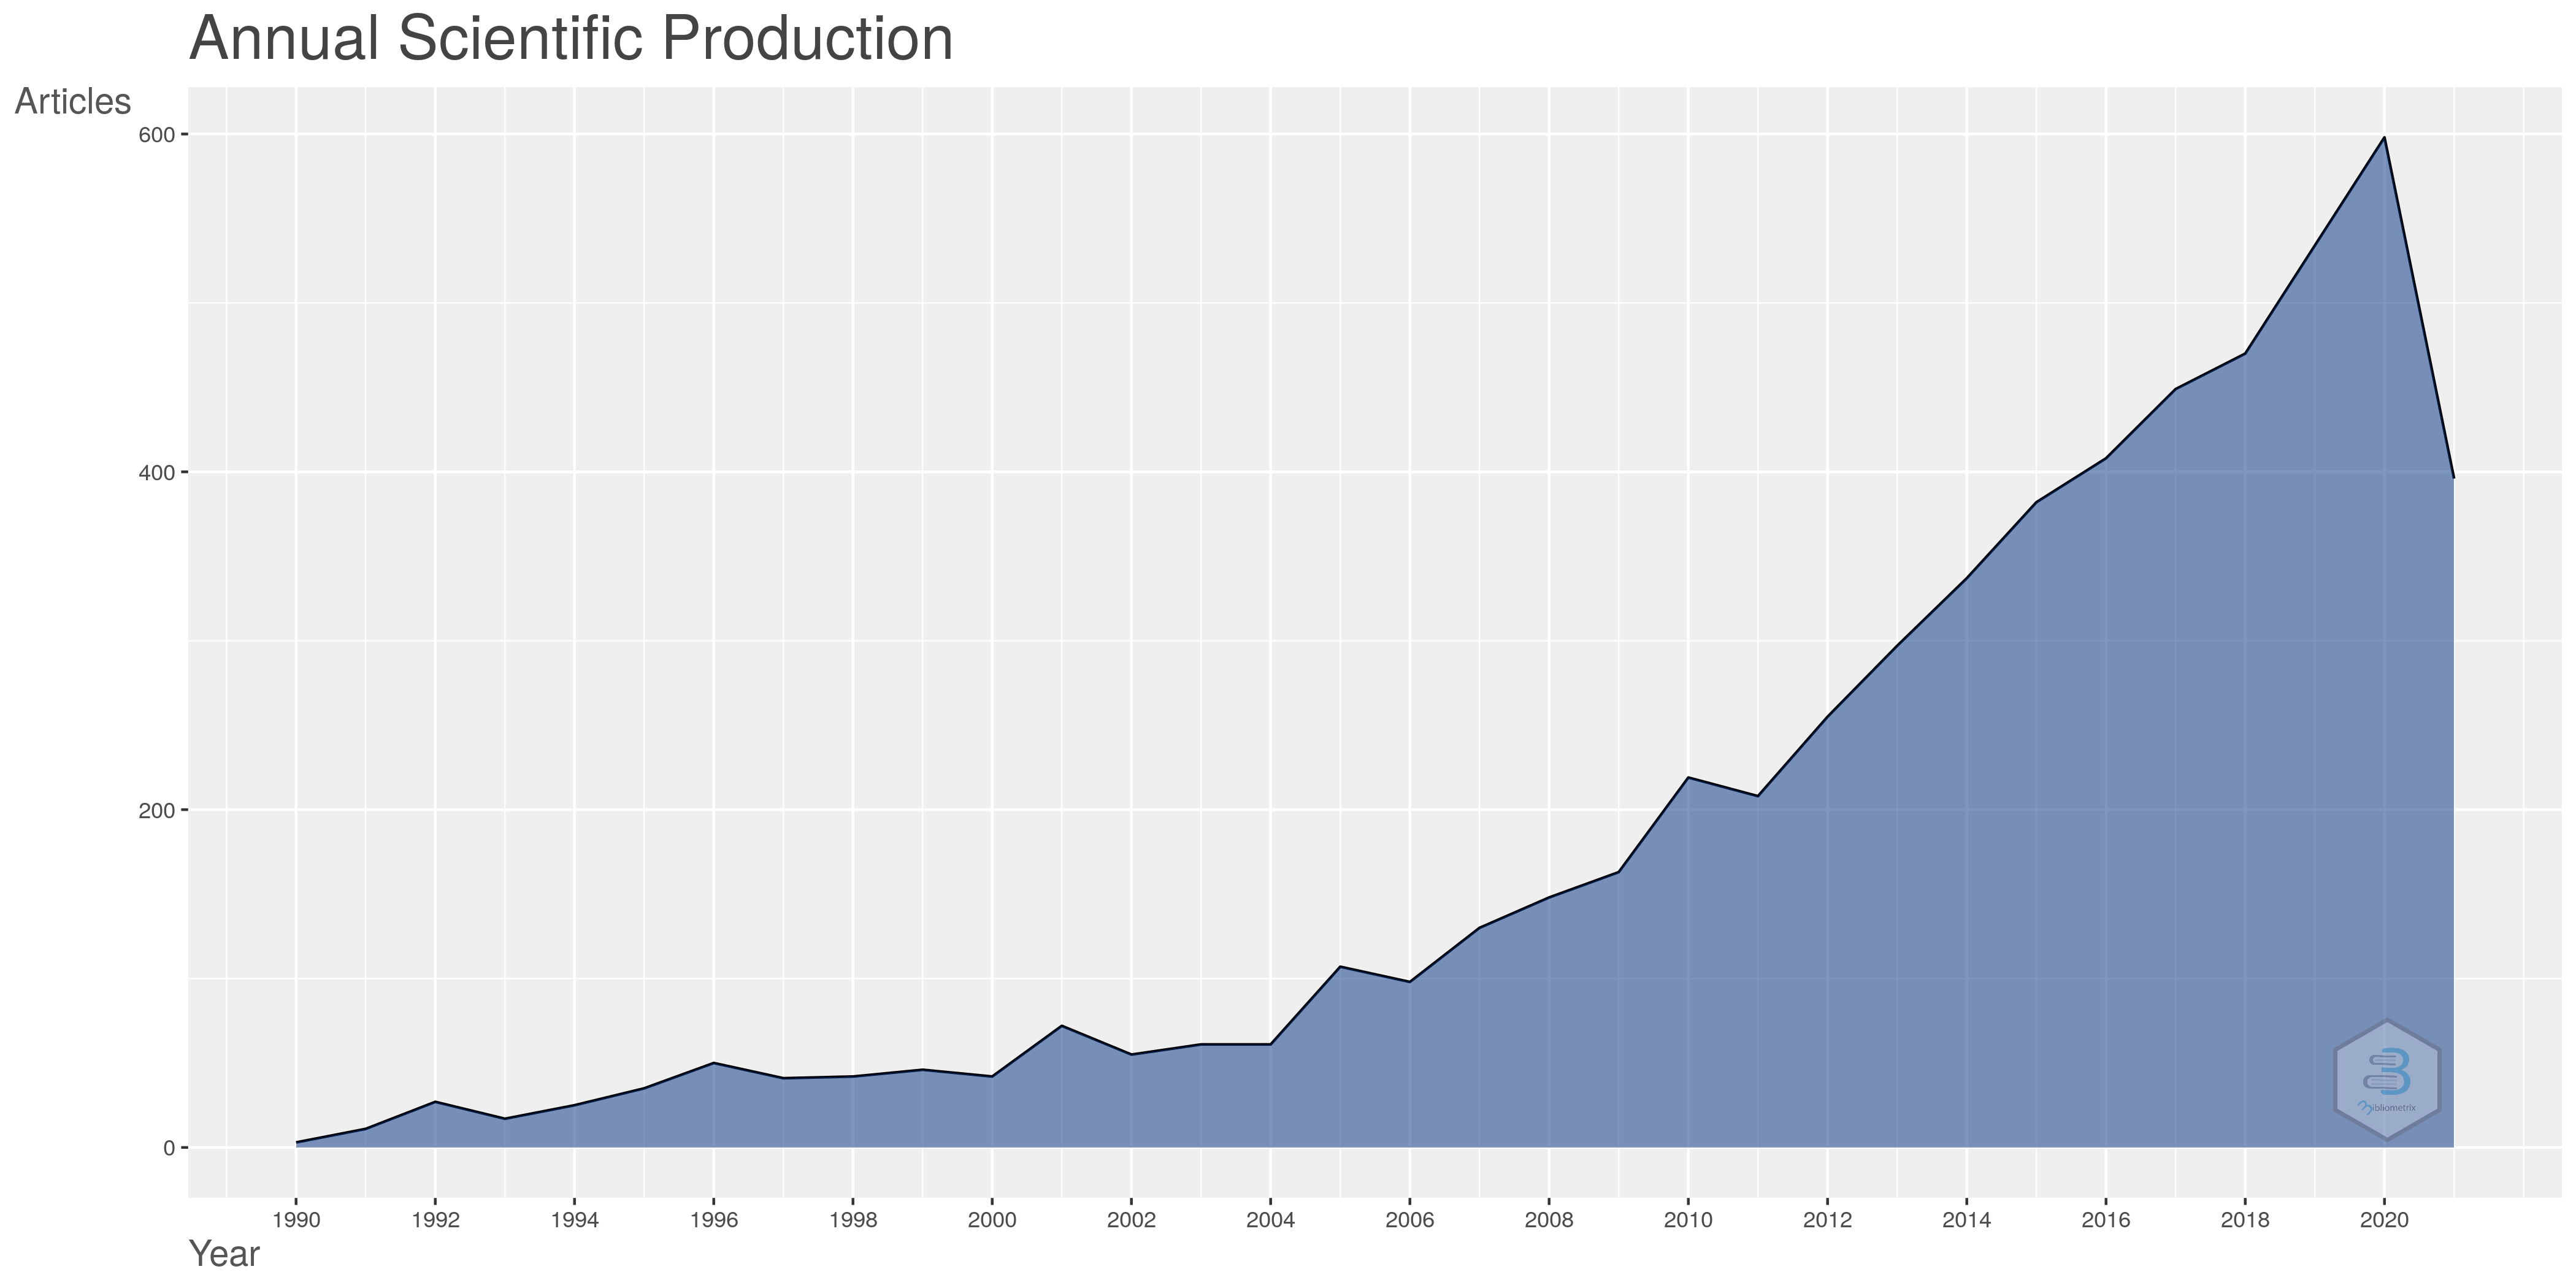
\includegraphics[width=1\textwidth]{experiments/jhcf/PesqBibliogr/SimulacaoMultiagente/WoS-20210803/classico-mais-citacoes/Dataset/AnnualScientificProduction-2021-08-05.png}
    \caption{Evolução da produção científica no dataset MASSA@jhcf.}
    \label{fig:evol:anual:MASSA@jhcf}
\end{figure}

A figura \ref{fig:evol:anual:MASSA@jhcf} apresenta a evolução da produção científica mundial no tema de interesse, segundo o dataset MASSA@jhcf. A curva mostra uma tendência de crescimento aproximadamente exponencial da quantidade de publicações, desde a primeira identificada em 1990.

O \textit{Annual Growth Rate} do dataset é de 17,06\%, bem maior que a taxa média de crescimento da publicação científica mundial, de cerca de 3,3\% anuais, em 2016, como ilustra o estudo em \url{https://www.researchgate.net/publication/333972683_Dynamics_of_scientific_production_in_the_world_in_Europe_and_in_France_2000-2016}, página 23.

\subsection{Interpretação do Crescimento} A maior taxa de crescimento do dataset MASSA@jhcf, bem como o seu grande volume, sugerem que o assunto em pauta desperta intenso interesse, inclusive de ordem econômica.

\subsection{Evolução das Citações}

\begin{figure}
    \centering
    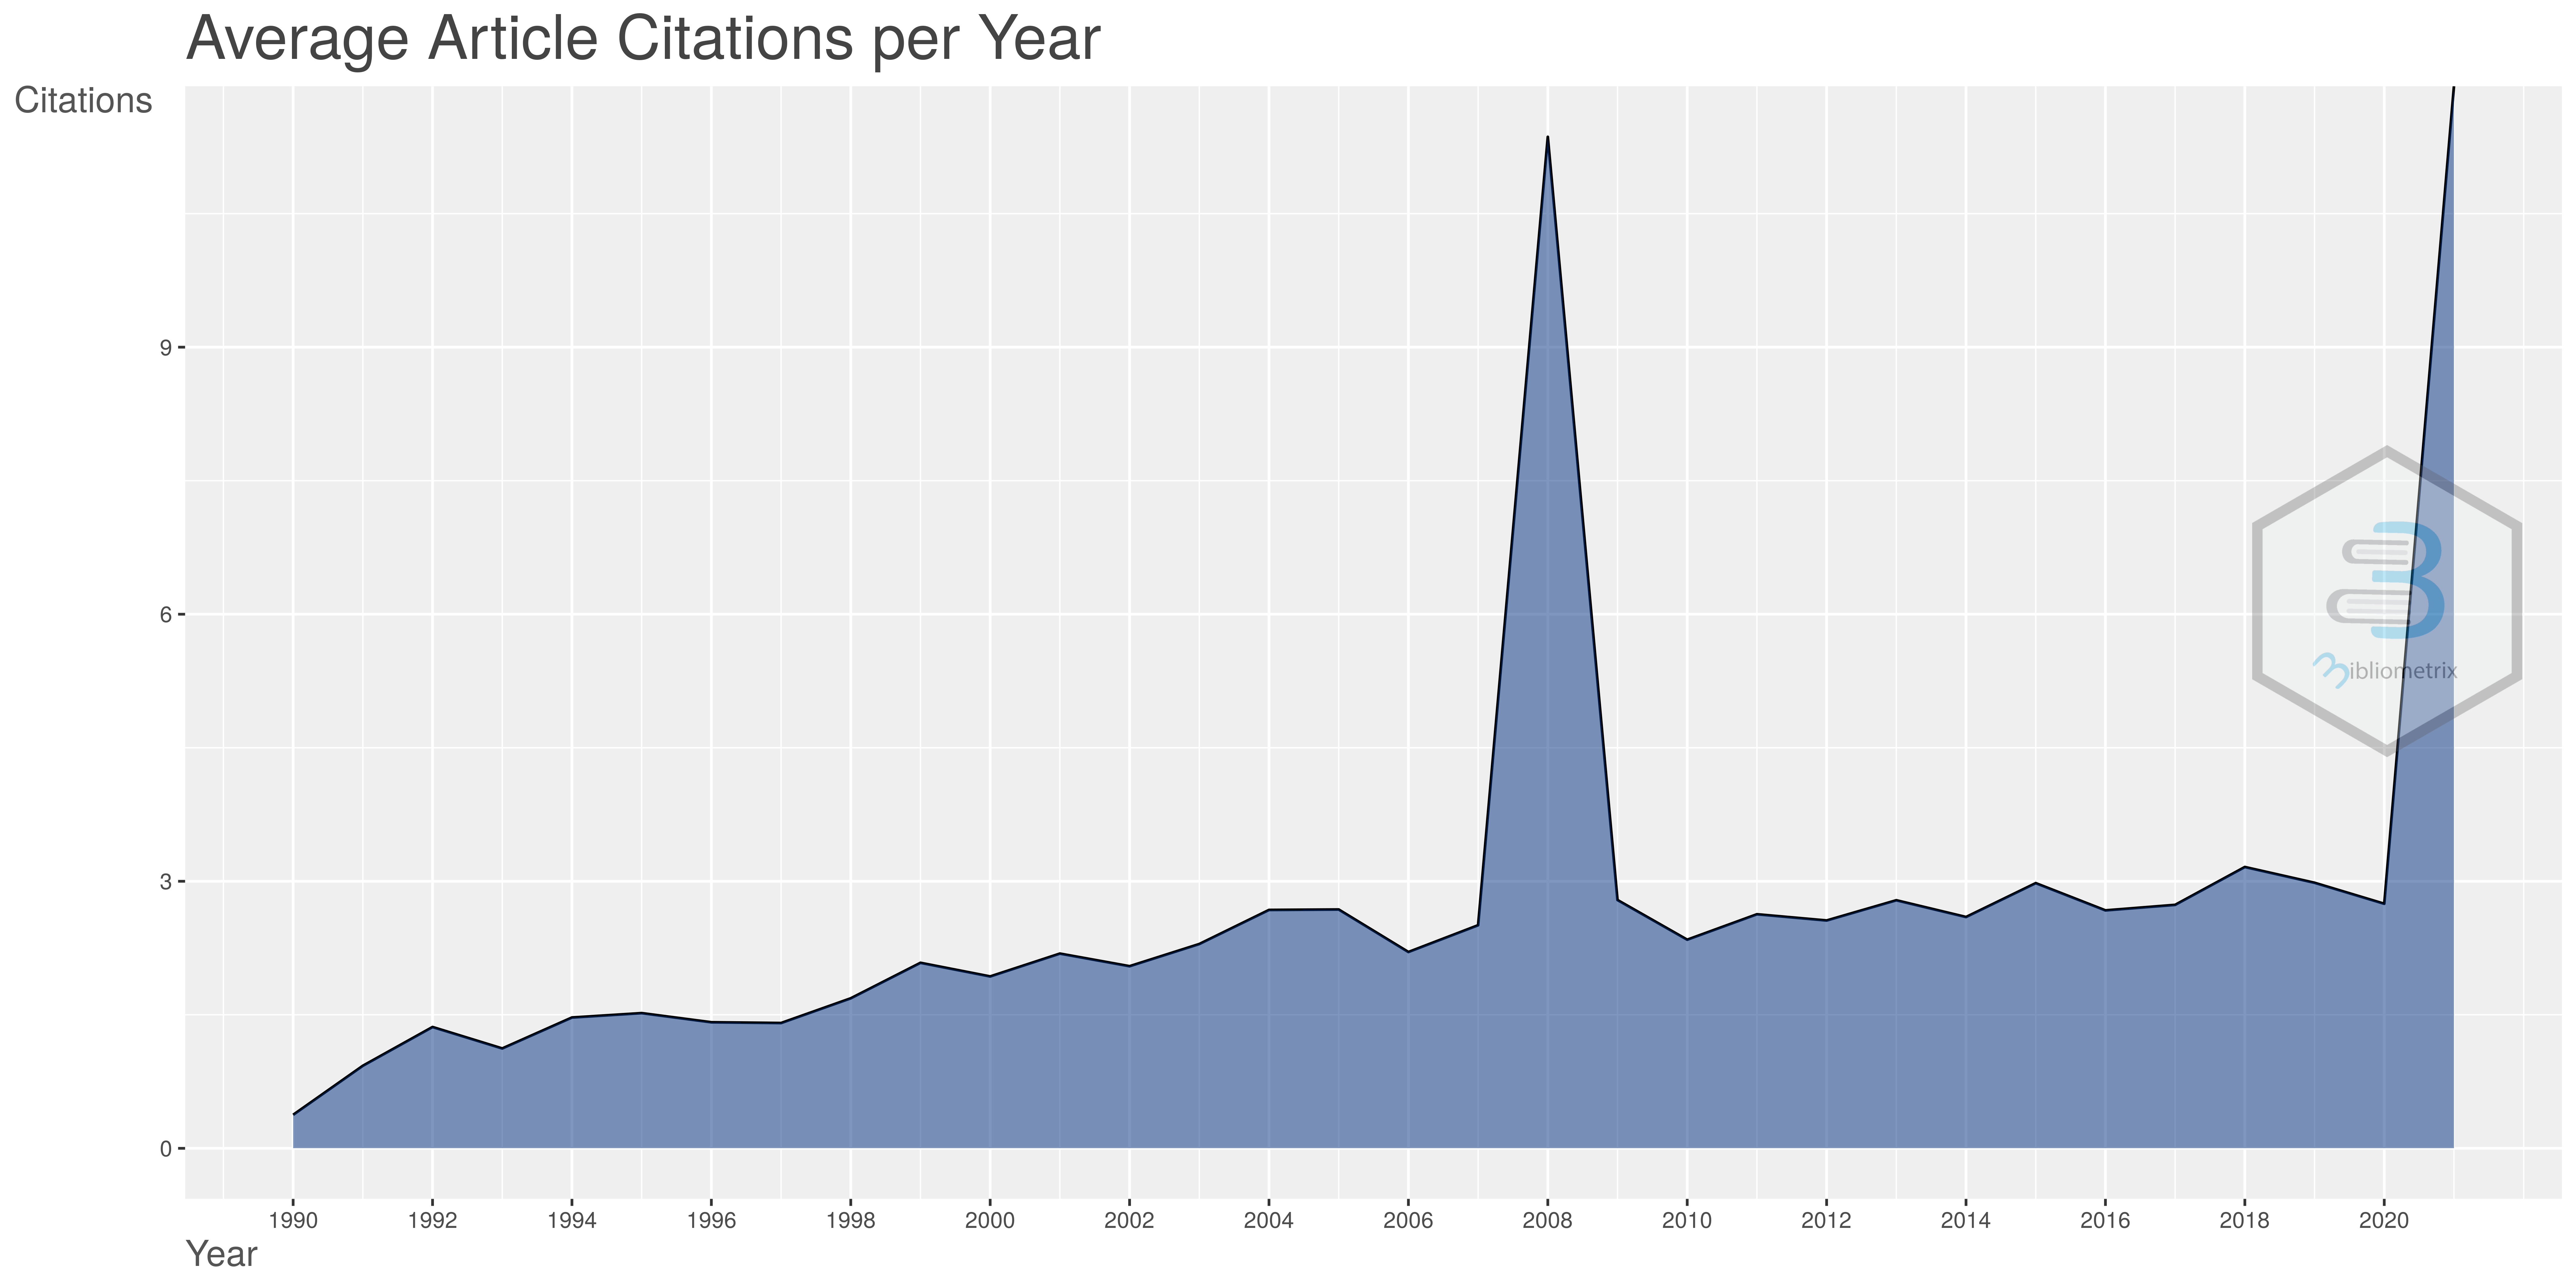
\includegraphics[width=1\textwidth]{experiments/jhcf/PesqBibliogr/SimulacaoMultiagente/WoS-20210803/classico-mais-citacoes/Dataset/AverageArticleCitationPerYear-2021-08-09.png}
    \caption{Evolução das citações ao dataset MASSA@jhcf.}
    \label{fig:evol:anual:citacoes:MASSA@jhcf}
\end{figure}

A figura \ref{fig:evol:anual:citacoes:MASSA@jhcf} apresenta a evolução da média de citações aos 5.787 artigos no dataset MASSA@jhcf. 
Nota-se grande estabilidade na média anual de citações, onde os artigos publicados em 1992 possuem cerca de 2 citações médias, e em 2015 (17 anos depois) o valou alterou-se apenas para três. O pico que aparece no ano de 2008 deve-se, possivelmente, à presença de um artigo do dataset, publicado em 2008, que possui um número surpreendente grande de citações. \footnote{Note que o cálculo do número  médio de citações, nesse caso, utiliza os valores computados no tag "TC (Times Cited)", já presentes no dataset obtido. Ou seja, o gráfico baseia-se no número de citações globais (externas ao dataset MASSA@jhcf), e não no número de citações locais (citações a um artigo do dataset feitas por alguns dos outros artigos dentro do próprio dataset).}.

\subsection{Interpretação das Citações}
Mesmo perante um crescimento aproximadamente exponencial no volume de publicações, a ocorrência de um crescimento nas citações médias ao longo dos anos sugere que os artigos do dataset possuem uma tendência de crescimento no tamanho da bibliografia citada, bem como também despertam grande interesse dos cientistas nas demais áreas do conhecimento (já que se trata de citações globais).

\subsection{\textit{Three-Field Plots (Sankey diagram)}}

As \textit{Three-Field Plots (Sankey diagram)} (plotagens do tipo ``Três Campos'') apresentam afinidades entre três conjuntos de atributos agregados que ocorrem no dataset. Uma plotagem do tipo Sankey busca mostrar os principais fluxos entre diferentes conjuntos de itens. \footnote{Para uma introdução ver \url{https://en.wikipedia.org/wiki/Sankey_diagram}. Para obter detalhes sobre a forma de geração e utilização desse gráfico, inclusive de forma interativa, veja o vídeo em \url{https://www.youtube.com/watch?v=jBb1iha6-sg}.} 

\begin{figure}
    \centering
    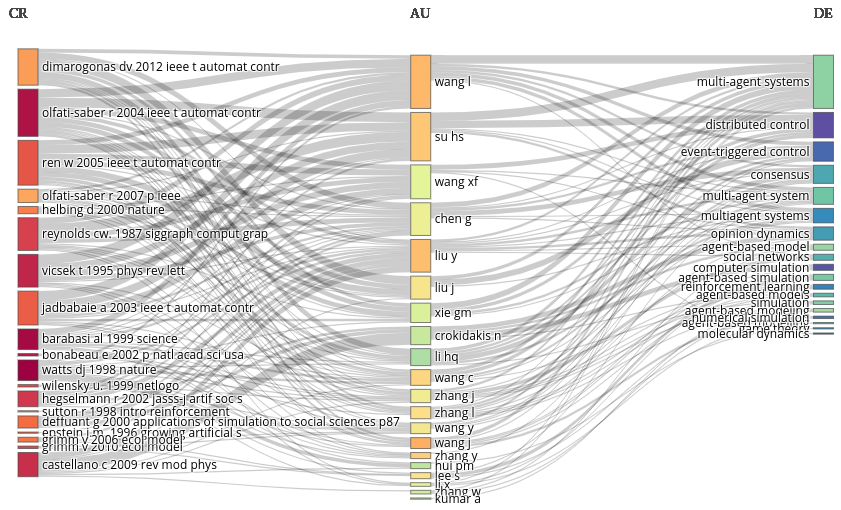
\includegraphics[angle=0,width=1\textwidth]{experiments/jhcf/PesqBibliogr/SimulacaoMultiagente/WoS-20210803/classico-mais-citacoes/Dataset/ThreeFieldPlot-AU-CR-DE-20-20-20.png}
    \caption{Plotagem ``Três Campos'' (Sankey plot) do dataset MASSA@jhcf: 20 Autores, Citações e Palavras-Chave mais proeminentes.}
    \label{fig:MASSA@jhcf:ThreeFieldPlot}
\end{figure}

A figura \ref{fig:MASSA@jhcf:ThreeFieldPlot} apresenta a plotagem do tipo ``Três Campos'' do dataset MASSA@jhcf, vinculando, ao centro, os 20 Autores mais proeminentes (AU), à esquerda, as 20 Citações mais frequentes (CR - Cited Records), e à direita, as 20 Palavras-Chave mais frequentes empregadas pelos autores.

\subsection{Interpretação da figura \ref{fig:MASSA@jhcf:ThreeFieldPlot}}
Os vinte autores mais relevantes, em relação aos artigos mais relevantes citados, e as palavras-chave mais relevantes são aparentemente de origem asiática, mais especificamente chinesa, com base nos sobrenomes. De outra formal, a mesma origem chinesa parece não se aplicar aos trabalhos mais citados, aparentemente europeus ou norte-americanos. Isso sugere estar ocorrendo uma migração recente da produção científica, do ocidente para o oriente. 

Adicionalmente, dentre as palavras-chave (DE) não relacionadas diretamente aos termos de busca, emergem os termos \textbf{distributed control}, \textbf{event-triggered control}, \textbf{consensus} e \textbf{opinion dynamics}. Isso sugere foco das pesquisas por autores de origem chinesa no uso de simulação multiagente voltada à compreensão dos fenômenos de controle social distribuído, formação de consenso e dinâmica da opinião (pública?).

Ainda sobre a interpretação da plotagem da figura \ref{fig:MASSA@jhcf:ThreeFieldPlot}, observa-se que os artigos mais citados encontram-se publicados pelo menos 10 anos atrás, sugerindo que não houve, nos últimos 10 anos, nenhum trabalho que tenha produzido uma mudança de paradigma no tema.
A fim de melhor evidenciar as citações mais relevantes segundo o peso dos autores e palavras-chave, o gráfico da figura \ref{fig:MASSA@jhcf:ThreeFieldPlot:10-20-20} plota apenas as 10 referências citadas, para 20 autores e palavras-chave mais proeminentes.

\begin{figure}
    \centering
    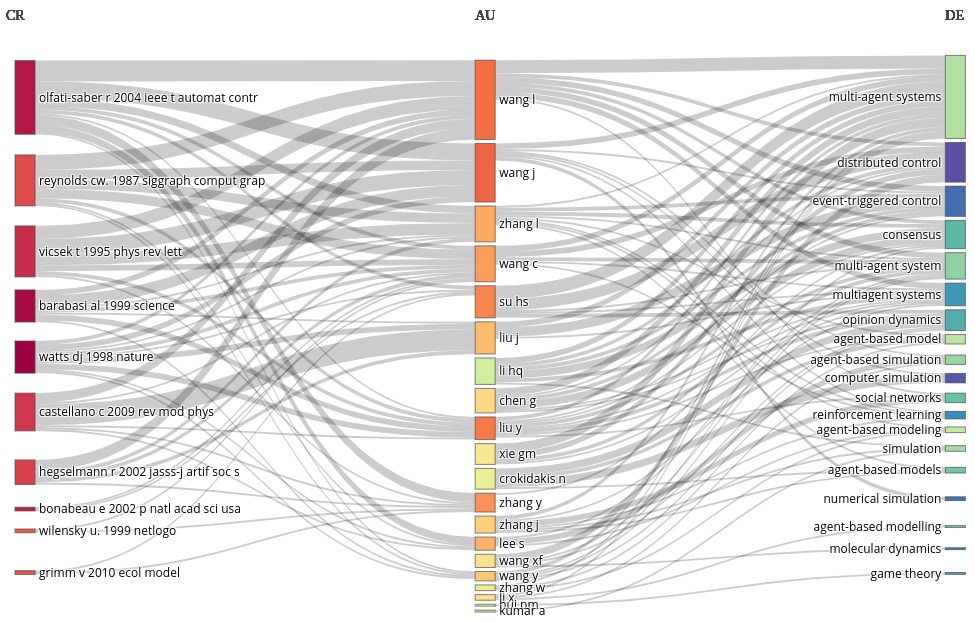
\includegraphics[angle=0,width=1\textwidth]{experiments/jhcf/PesqBibliogr/SimulacaoMultiagente/WoS-20210803/classico-mais-citacoes/Dataset/ThreeFieldPlot-AU-CR-DE-20-10-20.png}
    \caption{Plotagem ``Três Campos'' (Sankey plot) do dataset MASSA@jhcf: 10 Autores, 20 Citações e Palavras-Chave mais proeminentes.}
    \label{fig:MASSA@jhcf:ThreeFieldPlot:10-20-20}
\end{figure}

Breves comentários sobre cada um desses trabalhos serão tratados em seção posterior.

\begin{itemize}
    \item  \cite{olfati-saber_consensus_2004} apresentam discussões teóricas sobre a formação de consenso em sistemas multi-agentes com topologias variáveis;
    \item  \cite{reynolds_flocks_1987} apresenta modelos multi-agentes para simulação gráfica do movimento de rebanhos ou agregados de animais.
    \item \cite{vicsek_novel_1995} analisam a emergência de fenômenos de transição de fase em simulações de de partículas com comportamento autônomo com interação biologicamente motivada.
    \item \cite{barabasi_emergence_1999} investigam a emergência da distribuição livre de escala (\textit{scale-free}\footnote{Ver introdução em \url{https://en.wikipedia.org/wiki/Scale-free_network}.}) em redes que evoluem com base em ligação preferencial.
    \item \cite{watts_collective_1998} exploram o surgimento de redes do tipo mundo pequeno (\textit{small world}\footnote{Ver introdução em \url{https://en.wikipedia.org/wiki/Small-world_network}.}) formadas a partir da reorganização aleatória de redes biológicas, genéticas e outras formas de redes auto-organizadas.
    \item \cite{castellano_statistical_2009} exploram de que forma as técnicas de análise e simulação já usadas na física-estatística podem ser usadas para explicar vários fenômenos sociais, tais como comportamento de multidões, dispersão social, comportamento de multidões etc. Eles apresentam as afinidades entre os dados gerados pelos modelos simulados e dados empíricos obtidos junto a sistemas sociais reais. 
    \item \cite{hegselmann_opinion_2002} exploram a emergência de fenômenos de consenso, polarização e fragmentação da opinião na simulação de sociedades artificiais.
    \item \cite{bonabeau_agent-based_2002} apresenta os potenciais e campos de aplicação da técnicas de simulação baseada em agentes.
    \item \cite{wilensky_netlogo_1999} apresentam a linguagem e ambiente de simulação NetLogo.
    \item \cite{grimm_standard_2006} apresenta o protocolo ODD, proposto para padronizar a descrição de modelos de simulação multiagente.
\end{itemize}

Nenhum desses 10 documentos citados está contido no dataset recuperado.

\subsection{Análises Bibliométricas: Fontes de Informação}

\begin{figure}
    \centering
%    \includegraphics[angle=0,width=1\textwidth]{}
    \caption{Plotagem ``Três Campos'' (Sankey plot) do dataset MASSA@jhcf: 20 Autores, Citações e Palavras-Chave mais proeminentes.}
    \label{fig:MASSA@jhcf:ThreeFieldPlot}
\end{figure}

\subsection{Análises Bibliométricas: Autores}

\subsection{Análises Bibliométricas: Documentos}

